\documentclass[11pt]{article}

\usepackage[margin=1in]{geometry}
\usepackage{amsmath,amssymb,mathtools}
\usepackage{tikz}
\usetikzlibrary{arrows.meta,calc}
\usepackage{enumitem}
\usepackage[hidelinks]{hyperref}
\usepackage{microtype}

\setlength{\parindent}{0pt}
\setlength{\parskip}{0.65em}
\setlist[itemize]{leftmargin=2em,itemsep=0.3em,topsep=0.3em}
\setlist[enumerate]{leftmargin=2.2em,itemsep=0.4em,topsep=0.4em}

\newcommand{\R}{\mathbb{R}}
\newcommand{\GM}{\operatorname{GM}}

\title{A High-School-Friendly Tutorial\\[0.25em]
Exercise 8.5: The Geometric Mean as a Minimum}
\author{}
\date{}

\begin{document}
\maketitle
\tableofcontents
\bigskip

\section{What the Exercise Is Asking}

The exercise has two connected parts.

\begin{enumerate}
\item Prove that the geometric mean of positive numbers
\[
 a_1,a_2,\ldots,a_n
\]
can be obtained by minimizing a certain weighted arithmetic mean.

\item Use that minimum formula to prove that the geometric mean is
\emph{superadditive}.
\end{enumerate}

For a positive vector
\[
 \mathbf a=(a_1,a_2,\ldots,a_n),
\]
define its geometric mean by
\[
 \GM(\mathbf a)
 =\left(\prod_{k=1}^{n}a_k\right)^{1/n}.
\]
The region in the exercise is
\[
 D=
 \left\{
 (x_1,x_2,\ldots,x_n)\in\R^n:
 x_k\ge 0\text{ for every }k,
 \ \prod_{k=1}^{n}x_k=1
 \right\}.
\]
The first statement to prove is
\begin{equation*}
\boxed{
 \GM(\mathbf a)
 =
 \min_{\mathbf x\in D}
 \frac1n\sum_{k=1}^{n}a_kx_k.
}
\tag{8.33}
\end{equation*}

The second statement, called superadditivity, is
\begin{equation*}
\boxed{
 \left(\prod_{k=1}^{n}(a_k+b_k)\right)^{1/n}
 \ge
 \left(\prod_{k=1}^{n}a_k\right)^{1/n}
 +
 \left(\prod_{k=1}^{n}b_k\right)^{1/n}.
}
\tag{SA}
\end{equation*}
Here the two lists are added coordinate by coordinate:
\[
 \mathbf a+\mathbf b
 =(a_1+b_1,a_2+b_2,\ldots,a_n+b_n).
\]

\paragraph{Positivity assumption.}
For the main proof, we assume
\[
 a_k>0\quad\text{and}\quad b_k>0
 \qquad(k=1,2,\ldots,n).
\]
This is the case in which the right-hand side of (8.33) has an actual
minimum.  Section~\ref{sec:zeros} explains carefully what changes if zero
entries are allowed.

\section{Reading the Notation}

\subsection{Sum notation}

The symbol
\[
 \sum_{k=1}^{n}a_kx_k
\]
means
\[
 a_1x_1+a_2x_2+\cdots+a_nx_n.
\]
Therefore
\[
 \frac1n\sum_{k=1}^{n}a_kx_k
\]
is the arithmetic mean of the $n$ numbers
\[
 a_1x_1,a_2x_2,\ldots,a_nx_n.
\]

\subsection{Product notation}

The symbol
\[
 \prod_{k=1}^{n}a_k
\]
means
\[
 a_1a_2\cdots a_n.
\]
For example, when $n=3$,
\[
 \left(\prod_{k=1}^{3}a_k\right)^{1/3}
 =(a_1a_2a_3)^{1/3}.
\]

\subsection{What does the set D mean?}

A point $\mathbf x=(x_1,\ldots,x_n)$ belongs to $D$ when its coordinates have
product $1$:
\[
 x_1x_2\cdots x_n=1.
\]
Although the definition says $x_k\ge0$, the product condition automatically
forces every coordinate to be strictly positive.  Indeed, if one coordinate
were $0$, then the whole product would be $0$, not $1$.  Thus every
$\mathbf x\in D$ satisfies
\[
 x_k>0\qquad(k=1,2,\ldots,n).
\]

For $n=3$, some examples of points in $D$ are
\[
 (1,1,1),
 \qquad
 \left(2,\frac12,1\right),
 \qquad
 \left(2,2,\frac14\right).
\]
The coordinates may change, but their product must stay equal to $1$.

It is useful to think of the $x_k$ as \emph{adjusting factors}.  Making one
$x_k$ larger forces one or more of the others to become smaller so that the
total product remains $1$.

\subsection{What does a minimum proof require?}

Suppose we want to prove that the minimum of some expression is $g$.  There are
two separate jobs.

\begin{enumerate}
\item \textbf{Lower-bound job:} Show that every allowed choice gives a value at
least $g$.

\item \textbf{Attainment job:} Find one allowed choice that gives exactly $g$.
\end{enumerate}

The first job proves that the answer cannot be below $g$.  The second proves
that the answer is not above $g$.  Together they prove that the minimum is
exactly $g$.

\section{The Main Tool: the AM--GM Inequality}

For positive numbers $y_1,y_2,\ldots,y_n$, the arithmetic mean--geometric mean
inequality says
\begin{equation*}
\boxed{
 \frac{y_1+y_2+\cdots+y_n}{n}
 \ge
 (y_1y_2\cdots y_n)^{1/n}.
}
\tag{AM--GM}
\end{equation*}
Equality holds exactly when
\[
 y_1=y_2=\cdots=y_n.
\]

For example,
\[
 \frac{2+8}{2}=5
 \ge
 \sqrt{2\cdot8}=4.
\]
The arithmetic mean is larger because the numbers $2$ and $8$ are unequal.  If
we use two equal numbers, such as $4$ and $4$, then
\[
 \frac{4+4}{2}=4=\sqrt{4\cdot4}.
\]

A very important interpretation of AM--GM is this:

\begin{center}
\emph{Among positive numbers with a fixed product, the sum is smallest when the
numbers are all equal.}
\end{center}

That sentence is exactly the idea behind Exercise~8.5.

\section{Warm-Up: the Two-Number Case}

When $n=2$, the condition $x_1x_2=1$ lets us write
\[
 x_1=t,
 \qquad
 x_2=\frac1t,
 \qquad t>0.
\]
The claimed formula becomes
\[
 \sqrt{a_1a_2}
 =
 \min_{t>0}
 \frac12\left(a_1t+\frac{a_2}{t}\right).
\]
Apply AM--GM to the two positive numbers
\[
 a_1t
 \qquad\text{and}\qquad
 \frac{a_2}{t}.
\]
We get
\begin{align*}
 \frac12\left(a_1t+\frac{a_2}{t}\right)
 &\ge
 \sqrt{a_1t\cdot\frac{a_2}{t}}\\
 &=\sqrt{a_1a_2}.
\end{align*}
The variable $t$ disappears from the product because $t(1/t)=1$.

Equality in AM--GM occurs when the two adjusted terms are equal:
\[
 a_1t=\frac{a_2}{t}.
\]
Therefore
\[
 a_1t^2=a_2,
 \qquad
 t=\sqrt{\frac{a_2}{a_1}}.
\]
At this choice,
\[
 x_1=\sqrt{\frac{a_2}{a_1}},
 \qquad
 x_2=\sqrt{\frac{a_1}{a_2}}.
\]
Their product is $1$, so this point is allowed.

\subsection{A numerical example}

Let
\[
 a_1=4,
 \qquad
 a_2=9.
\]
The geometric mean is
\[
 \sqrt{4\cdot9}=6.
\]
The minimizing point is
\[
 x_1=\sqrt{\frac94}=\frac32,
 \qquad
 x_2=\sqrt{\frac49}=\frac23.
\]
The two adjusted terms are equal:
\[
 a_1x_1=4\cdot\frac32=6,
 \qquad
 a_2x_2=9\cdot\frac23=6.
\]
Hence
\[
 \frac{a_1x_1+a_2x_2}{2}
 =\frac{6+6}{2}=6.
\]

The next figure gives a geometric picture.  The curved line is the constraint
$x_1x_2=1$.  A straight line of the form
\[
 4x_1+9x_2=c
\]
contains points where the weighted sum has the same value.  Moving such a line
toward the origin makes $c$ smaller.  The smallest line that still touches the
constraint curve is tangent at
\[
 \left(\frac32,\frac23\right).
\]

\begin{figure}[htbp]
\centering
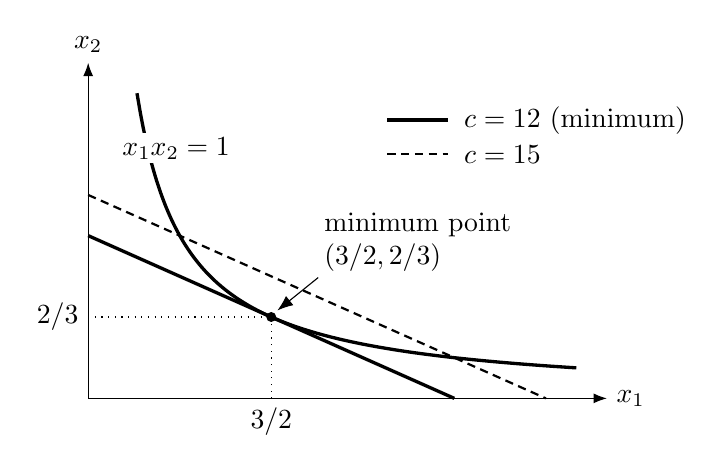
\begin{tikzpicture}[x=1.55cm,y=1.55cm,>=Latex]
  \draw[->] (0,0)--(4.25,0) node[right] {$x_1$};
  \draw[->] (0,0)--(0,2.75) node[above] {$x_2$};

  \draw[very thick,domain=0.4:4.0,samples=140,smooth,variable=\t]
       plot ({\t},{1/\t});
  \node[fill=white,inner sep=1.5pt] at (0.72,2.05) {$x_1x_2=1$};

  \draw[densely dashed,thick] (0,1.6667)--(3.75,0);
  \draw[very thick] (0,1.3333)--(3,0);

  \draw[very thick] (2.45,2.28)--(2.95,2.28);
  \node[right] at (3.00,2.28) {$c=12$ (minimum)};
  \draw[densely dashed,thick] (2.45,2.00)--(2.95,2.00);
  \node[right] at (3.00,2.00) {$c=15$};

  \fill (1.5,0.6667) circle (1.8pt);
  \draw[dotted] (1.5,0)--(1.5,0.6667);
  \draw[dotted] (0,0.6667)--(1.5,0.6667);
  \node[below] at (1.5,0) {$3/2$};
  \node[left] at (0,0.6667) {$2/3$};

  \node[fill=white,inner sep=2pt,align=left] (label) at (2.70,1.28)
       {minimum point\\$\left(3/2,2/3\right)$};
  \draw[-{Latex[length=2mm]}] (label.south west)--(1.55,0.72);
\end{tikzpicture}
\caption{For $a_1=4$ and $a_2=9$, the smallest level line that meets
$x_1x_2=1$ is $4x_1+9x_2=12$.  Dividing by $2$ gives the minimum value $6$.}
\end{figure}

\section{Complete Proof of the Minimum Representation}

Let
\[
 g=\GM(\mathbf a)
 =\left(\prod_{k=1}^{n}a_k\right)^{1/n}.
\]
We will carry out the two jobs described earlier.

\subsection{Step 1: every allowed value is at least the geometric mean}

Choose any point
\[
 \mathbf x=(x_1,x_2,\ldots,x_n)\in D.
\]
Because $a_k>0$ and $x_k>0$, the numbers
\[
 a_1x_1,a_2x_2,\ldots,a_nx_n
\]
are all positive.  Apply AM--GM to them:
\begin{align*}
 \frac1n\sum_{k=1}^{n}a_kx_k
 &\ge
 \left(\prod_{k=1}^{n}a_kx_k\right)^{1/n}\\
 &=
 \left(
   \left(\prod_{k=1}^{n}a_k\right)
   \left(\prod_{k=1}^{n}x_k\right)
 \right)^{1/n}\\
 &=
 \left(
   \left(\prod_{k=1}^{n}a_k\right)\cdot1
 \right)^{1/n}\\
 &=g.
\end{align*}
The third line used the defining property of $D$:
\[
 \prod_{k=1}^{n}x_k=1.
\]

This inequality is true for \emph{every} point $\mathbf x\in D$.  Therefore the
smallest possible value cannot be less than $g$:
\begin{equation*}
 \min_{\mathbf x\in D}
 \frac1n\sum_{k=1}^{n}a_kx_k
 \ge g.
\tag{1}
\end{equation*}

\subsection{Step 2: construct a point that gives exactly the geometric mean}

AM--GM becomes an equality when all its input numbers are equal.  We therefore
want
\[
 a_1x_1=a_2x_2=\cdots=a_nx_n=g.
\]
This suggests choosing
\begin{equation*}
\boxed{
 x_k^*=\frac{g}{a_k}
 \qquad(k=1,2,\ldots,n).
}
\tag{2}
\end{equation*}
Each $x_k^*$ is positive.  We must check that the product is $1$:
\begin{align*}
 \prod_{k=1}^{n}x_k^*
 &=\prod_{k=1}^{n}\frac{g}{a_k}\\
 &=\frac{g^n}{\prod_{k=1}^{n}a_k}\\
 &=\frac{\prod_{k=1}^{n}a_k}
         {\prod_{k=1}^{n}a_k}\\
 &=1.
\end{align*}
Here we used
\[
 g^n=\prod_{k=1}^{n}a_k.
\]
Thus $\mathbf x^*\in D$.

Now evaluate the objective at this point:
\begin{align*}
 \frac1n\sum_{k=1}^{n}a_kx_k^*
 &=\frac1n\sum_{k=1}^{n}a_k\frac{g}{a_k}\\
 &=\frac1n\sum_{k=1}^{n}g\\
 &=\frac1n(ng)\\
 &=g.
\end{align*}
So an allowed point actually gives the value $g$.  Therefore
\begin{equation*}
 \min_{\mathbf x\in D}
 \frac1n\sum_{k=1}^{n}a_kx_k
 \le g.
\tag{3}
\end{equation*}

Combining (1) and (3), we obtain
\[
 \boxed{
 \left(\prod_{k=1}^{n}a_k\right)^{1/n}
 =
 \min_{\mathbf x\in D}
 \frac1n\sum_{k=1}^{n}a_kx_k.
 }
\]
This proves formula (8.33).

\subsection{What is the minimizing point?}

The proof found the minimizer explicitly:
\[
 \boxed{
 \mathbf x^*
 =\left(
 \frac{g}{a_1},
 \frac{g}{a_2},
 \ldots,
 \frac{g}{a_n}
 \right).
 }
\]
At this point,
\[
 a_1x_1^*=a_2x_2^*=\cdots=a_nx_n^*=g.
\]
Thus the minimizing factors balance all the adjusted numbers perfectly.

Because equality in AM--GM requires all adjusted terms to be equal, this is the
only minimizing point when all $a_k$ are positive.

\subsection{A three-number example}

Take
\[
 \mathbf a=(1,4,16).
\]
Its geometric mean is
\[
 g=(1\cdot4\cdot16)^{1/3}=64^{1/3}=4.
\]
The minimizing factors are
\[
 \mathbf x^*
 =\left(\frac41,\frac44,\frac4{16}\right)
 =\left(4,1,\frac14\right).
\]
Their product is
\[
 4\cdot1\cdot\frac14=1,
\]
and the adjusted numbers are
\[
 1\cdot4=4,
 \qquad
 4\cdot1=4,
 \qquad
 16\cdot\frac14=4.
\]
Consequently,
\[
 \frac{1\cdot4+4\cdot1+16\cdot(1/4)}{3}
 =\frac{4+4+4}{3}=4.
\]

\section{Using the Formula to Prove Superadditivity}

Let
\[
 \mathbf a=(a_1,\ldots,a_n),
 \qquad
 \mathbf b=(b_1,\ldots,b_n),
\]
with all entries positive.  We want to prove
\[
 \GM(\mathbf a+\mathbf b)
 \ge
 \GM(\mathbf a)+\GM(\mathbf b).
\]

\subsection{A general fact about minima}

Suppose $F$ and $H$ are two functions defined on the same set $D$.  For every
$x\in D$,
\[
 F(x)\ge\min_{u\in D}F(u)
 \qquad\text{and}\qquad
 H(x)\ge\min_{u\in D}H(u).
\]
Adding gives
\[
 F(x)+H(x)
 \ge
 \min_{u\in D}F(u)+\min_{u\in D}H(u).
\]
Because this is true for every $x\in D$, it remains true after minimizing the
left-hand side:
\begin{equation*}
\boxed{
 \min_{x\in D}\bigl(F(x)+H(x)\bigr)
 \ge
 \min_{x\in D}F(x)+\min_{x\in D}H(x).
}
\tag{4}
\end{equation*}

The direction $\ge$ is important.  The function $F$ may prefer one minimizing
point, while $H$ may prefer a different one.  On the left, both functions must
use the same point $x$.

\subsection{Apply the general fact}

For $\mathbf x\in D$, define
\[
 F_{\mathbf a}(\mathbf x)
 =\frac1n\sum_{k=1}^{n}a_kx_k,
 \qquad
 F_{\mathbf b}(\mathbf x)
 =\frac1n\sum_{k=1}^{n}b_kx_k.
\]
Then
\begin{align*}
 F_{\mathbf a+\mathbf b}(\mathbf x)
 &=\frac1n\sum_{k=1}^{n}(a_k+b_k)x_k\\
 &=\frac1n\sum_{k=1}^{n}a_kx_k
   +\frac1n\sum_{k=1}^{n}b_kx_k\\
 &=F_{\mathbf a}(\mathbf x)+F_{\mathbf b}(\mathbf x).
\end{align*}
Using the minimum representation (8.33) and then inequality (4),
\begin{align*}
 \GM(\mathbf a+\mathbf b)
 &=\min_{\mathbf x\in D}
   F_{\mathbf a+\mathbf b}(\mathbf x)\\
 &=\min_{\mathbf x\in D}
   \bigl(F_{\mathbf a}(\mathbf x)+F_{\mathbf b}(\mathbf x)\bigr)\\
 &\ge
   \min_{\mathbf x\in D}F_{\mathbf a}(\mathbf x)
   +
   \min_{\mathbf x\in D}F_{\mathbf b}(\mathbf x)\\
 &=\GM(\mathbf a)+\GM(\mathbf b).
\end{align*}
Writing this without vector notation gives
\[
 \boxed{
 \left(\prod_{k=1}^{n}(a_k+b_k)\right)^{1/n}
 \ge
 \left(\prod_{k=1}^{n}a_k\right)^{1/n}
 +
 \left(\prod_{k=1}^{n}b_k\right)^{1/n}.
 }
\]
This is the superadditivity of the geometric mean.

\subsection{The same proof, written point by point}

Some readers find the following version even clearer.  Fix any
$\mathbf x\in D$.  Formula (8.33) says
\[
 \frac1n\sum_{k=1}^{n}a_kx_k\ge\GM(\mathbf a)
\]
and
\[
 \frac1n\sum_{k=1}^{n}b_kx_k\ge\GM(\mathbf b).
\]
Adding,
\[
 \frac1n\sum_{k=1}^{n}(a_k+b_k)x_k
 \ge
 \GM(\mathbf a)+\GM(\mathbf b).
\]
This is true for every $\mathbf x\in D$.  Therefore it is true for the
smallest possible left-hand side.  But that smallest possible left-hand side is
$\GM(\mathbf a+\mathbf b)$ by (8.33).  Hence
\[
 \GM(\mathbf a+\mathbf b)
 \ge
 \GM(\mathbf a)+\GM(\mathbf b).
\]

\subsection{A numerical check}

Let
\[
 \mathbf a=(1,4),
 \qquad
 \mathbf b=(9,1).
\]
Then
\[
 \GM(\mathbf a)=\sqrt{1\cdot4}=2,
 \qquad
 \GM(\mathbf b)=\sqrt{9\cdot1}=3.
\]
Also,
\[
 \mathbf a+\mathbf b=(10,5),
\]
so
\[
 \GM(\mathbf a+\mathbf b)
 =\sqrt{10\cdot5}
 =\sqrt{50}
 =5\sqrt2
 \approx7.07.
\]
Thus
\[
 7.07\ge2+3=5.
\]
The inequality is strict in this example.

\subsection{When does equality occur?}

For positive entries, equality occurs exactly when the two vectors are
proportional.  This means that there is a positive constant $c$ such that
\[
 \mathbf a=c\mathbf b,
\]
or equivalently,
\[
 \frac{a_1}{b_1}
 =\frac{a_2}{b_2}
 =\cdots
 =\frac{a_n}{b_n}.
\]

Here is the reason.  The minimizing point for $\mathbf a$ is
\[
 x_k^{(a)}=\frac{\GM(\mathbf a)}{a_k},
\]
while the minimizing point for $\mathbf b$ is
\[
 x_k^{(b)}=\frac{\GM(\mathbf b)}{b_k}.
\]
For equality in the superadditivity proof, the same point must minimize both
expressions.  Therefore
\[
 \frac{\GM(\mathbf a)}{a_k}
 =\frac{\GM(\mathbf b)}{b_k}
 \qquad\text{for every }k,
\]
which says that $a_k/b_k$ is independent of $k$.

For example, take
\[
 \mathbf a=(1,4),
 \qquad
 \mathbf b=(2,8)=2\mathbf a.
\]
Then
\[
 \GM(\mathbf a)=2,
 \qquad
 \GM(\mathbf b)=4,
\]
and
\[
 \GM(\mathbf a+\mathbf b)
 =\GM(3,12)
 =\sqrt{36}=6=2+4.
\]

\section{Why the Minimum Representation Is So Useful}

The original geometric mean
\[
 \left(\prod_{k=1}^{n}a_k\right)^{1/n}
\]
contains a product and an $n$th root.  Those operations can be difficult to
handle when we add two vectors.

Formula (8.33) rewrites the same quantity as a minimum of expressions that are
linear in the entries $a_k$:
\[
 \frac1n\sum_{k=1}^{n}a_kx_k.
\]
Linear expressions split perfectly over addition:
\[
 \sum_{k=1}^{n}(a_k+b_k)x_k
 =\sum_{k=1}^{n}a_kx_k
 +\sum_{k=1}^{n}b_kx_k.
\]
That simple splitting is the entire reason the superadditivity proof becomes
short.

A useful summary is
\[
 \boxed{
 \text{fixed product constraint}
 \ +\ \text{AM--GM}
 \ \Longrightarrow\ \text{minimum formula}
 \ \Longrightarrow\ \text{superadditivity}.
 }
\]

\section{Technical Note About Zero Entries}
\label{sec:zeros}

The exercise writes ``minimum.''  This is correct when all $a_k>0$.  If some,
but not all, of the $a_k$ are zero, then the geometric mean is $0$, but the
minimum on the right usually is not attained.

For the simplest example, take $n=2$ and
\[
 (a_1,a_2)=(0,1).
\]
Every point in $D$ has the form $(t,1/t)$ with $t>0$, and
\[
 \frac12\left(a_1t+a_2\frac1t\right)
 =\frac1{2t}.
\]
As $t$ becomes larger and larger,
\[
 \frac1{2t}\longrightarrow0.
\]
The values can get arbitrarily close to $0$, but they never equal $0$ for a
finite positive $t$.  Therefore there is no minimum; there is only an
\emph{infimum}, meaning the greatest lower bound.

For nonnegative inputs, the completely general formula is
\[
 \boxed{
 \left(\prod_{k=1}^{n}a_k\right)^{1/n}
 =
 \inf_{\mathbf x\in D}
 \frac1n\sum_{k=1}^{n}a_kx_k.
 }
\]
When all $a_k>0$, the infimum is attained at $x_k=g/a_k$, so it is an actual
minimum.  The superadditivity proof works with $\inf$ in exactly the same way.
One may also prove the positive case first and then approach zero entries by a
limit.

\section{Common Mistakes to Avoid}

\begin{itemize}
\item \textbf{Forgetting that the product constraint matters.}
The cancellation
\[
 \prod_{k=1}^{n}a_kx_k
 =\left(\prod_{k=1}^{n}a_k\right)
  \left(\prod_{k=1}^{n}x_k\right)
 =\prod_{k=1}^{n}a_k
\]
works only because $\prod x_k=1$.

\item \textbf{Proving only a lower bound.}
Showing that every value is at least $g$ does not by itself prove that the
minimum equals $g$.  One must also exhibit the point $x_k=g/a_k$.

\item \textbf{Choosing the factors in the wrong direction.}
Large $a_k$ need small $x_k$, and small $a_k$ need large $x_k$.  The correct
choice is $x_k=g/a_k$, not $x_k=a_k/g$.

\item \textbf{Reversing the minimum inequality.}
In general,
\[
 \min(F+H)\ge\min F+\min H,
\]
not the other way around.

\item \textbf{Thinking that $x_k=0$ is allowed.}
The notation says $x_k\ge0$, but the condition $\prod x_k=1$ rules out zero.

\item \textbf{Ignoring the issue of zero coefficients.}
If some $a_k=0$, the general statement uses an infimum unless the surrounding
text has already assumed all $a_k>0$.
\end{itemize}

\section{The Two Proofs in Compact Form}

\textbf{Minimum representation.}
For every $\mathbf x\in D$, AM--GM gives
\[
 \frac1n\sum_{k=1}^{n}a_kx_k
 \ge
 \left(\prod_{k=1}^{n}a_kx_k\right)^{1/n}
 =
 \left(\prod_{k=1}^{n}a_k\right)^{1/n}.
\]
Equality is obtained by choosing
\[
 x_k=\frac{(\prod_{j=1}^{n}a_j)^{1/n}}{a_k}.
\]
Therefore (8.33) holds.

\textbf{Superadditivity.}
For every $\mathbf x\in D$,
\begin{align*}
 \frac1n\sum_{k=1}^{n}(a_k+b_k)x_k
 &=\frac1n\sum_{k=1}^{n}a_kx_k
   +\frac1n\sum_{k=1}^{n}b_kx_k\\
 &\ge\GM(\mathbf a)+\GM(\mathbf b).
\end{align*}
Taking the minimum over $D$ on the left gives
\[
 \GM(\mathbf a+\mathbf b)
 \ge\GM(\mathbf a)+\GM(\mathbf b).
\]

\section*{Quick Self-Check}

\begin{enumerate}
\item Why is every coordinate of a point in $D$ actually positive?\\
\emph{Answer:} If any coordinate were zero, the product of all coordinates
would be zero instead of one.

\item Which $n$ positive numbers receive AM--GM in the main proof?\\
\emph{Answer:} The adjusted numbers $a_1x_1,a_2x_2,\ldots,a_nx_n$.

\item Why does their product not depend on the chosen point $\mathbf x\in D$?\\
\emph{Answer:}
\[
 \prod(a_kx_k)=(\prod a_k)(\prod x_k)=\prod a_k
\]
because $\prod x_k=1$.

\item What choice makes equality hold in AM--GM?\\
\emph{Answer:}
\[
 x_k=\frac{g}{a_k},
 \qquad
 g=(\prod a_j)^{1/n},
\]
so that every adjusted term $a_kx_k$ equals $g$.

\item Why is $\min(F+H)$ usually not equal to $\min F+\min H$?\\
\emph{Answer:} The two functions may achieve their separate minima at different
points, while $F+H$ must use one common point.

\item What does superadditivity say in words?\\
\emph{Answer:} The geometric mean of the coordinatewise sum is at least the sum
of the two separate geometric means.
\end{enumerate}

\end{document}
